%!TEX root = ./main.tex
%!TEX encoding = UTF-8 Unicode
\chapter{Modeling the Instruction Set}
\section{Modeling using 3 views}
\label{sec:modelisationArborescente}
\subsection{Tree modeling approach}
\harmless\ uses 3 views to describe the instruction set of a processor:
\begin{itemize}
\item the binary view (\emph{format}) is used to describe the binary format of instruction to enable the decoding stage of instructions
\item the behavioral view (\emph{behavior}) allows to describe the behavior of instructions to simulate instructions.
\item the syntax view (\emph{syntax}) allows to describe the mnemonic of instruction to generate the disassembler.
\end{itemize}

Each view is a set of tree where each node describes a portion of \emph{format}, \emph{behavior} or \emph{syntax}. The description of a node is as follows:
\begin{verbatim}
<kind> <name> <kind_options>
  <kind_body>
end <kind>
\end{verbatim}
where \texttt{<kind>} can be \texttt{format}, \texttt{behavior} or \texttt{syntax}. By default, a node aggregates the sub nodes which are defined in the body. However, using the keyword \texttt{select}, a node may be chosen among others in the description of each trees.

This tree approach aims to factor up similar items (for the syntax, behavior or binary format). In each view, an instruction is represented by a branch in a tree. Instructions that share certain characteristics in a view share the same nodes.

\subsection{Instruction identification}
\label{sec:signature}
A node can have one or more \emph{tags}. A tag is represented in  \harmless\ using the \texttt{\#} character, followed by an alphanumerical string.
The \emph{set} of \emph{tags} along a branch of a tree is the unique identifier of an instruction and is called the \texttt{Instruction Identification.} The identification is a \emph{set}, which means that there is no order and no counting of the number of occurrence of each tags.

In some cases, it is useful to \emph{mark} tags, because the same node can be used in different contexts. For instance, when reading 2 source registers and one destination register, we use \emph{extended-tags}. An \emph{extended-tag} is represented using the \texttt{@} character, followed by an alphanumerical character string. As a consequence, each tags in the subtree are modified by adding the \emph{extended-tag} as a suffix (without the \texttt{@} character).

This mechanism is used to link instruction between the different views (format, syntax and behavior).

\subsection{An example}
\label{exempleSignature}
More detailled examples are given in the chapters associated to each views. The goal here is to show how is described the tree structure.
Consider for example the following (simplified) code:

\begin{lstlisting}
behavior readGPR #read8
  ...
end behavior

behavior writeGPR #write8
  ...
end behavior

-- instruction that operate on 2 source registers
behavior twoRegsOp
  -- read the 2 source registers
  readGPR@src1
  readGPR@src2
  select
    case #ADC  ...
    case #ADD  ...
    case #SUB  ...
  end select
  writeGPR
end behavior
\end{lstlisting}
This example describe 3 \texttt{behavior} nodes (non terminal):  \texttt{readGPR}, \texttt{writeGPR}, and \texttt{twoRegsOp}. The node \texttt{twoRegsOp} is the root, because it is not called by any other node. 

\begin{figure}		%% Small Example
  \begin{center}
    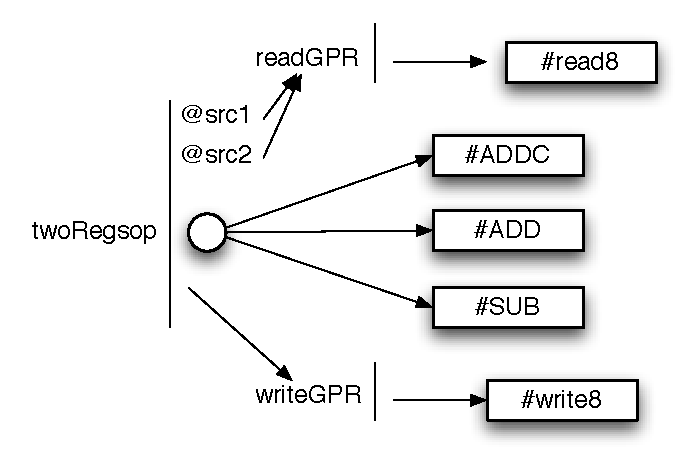
\includegraphics[width=0.8 \linewidth]{../common/images/instBase.pdf}
    \caption{Tree representation of the simple example.}
    \label{fig:instBase}
  \end{center}
\end{figure}

It is graphically represented in figure \ref{fig:instBase}. Each node is represented by name and by a vertical bar. To the right of the vertical bar, the various "elements" (selection, call for another node with or without \emph{extended-tag}) are shown \emph{sequentially}. The circle represent the structure of selection (\texttt{select}). Tags are represented in rectangles, and extended-tegs are represented in the calling node.

The advantage of using one extended-tag here lies in the fact that the \texttt{readGPR} node is called in 2 different contexts: one for each source register. As the extended-tag is added to each tags in the subtree, there are differentiated: \texttt{\#read8src1} and \texttt{\#read8src2}.

So in this example, the ADD instruction as a set of tags:  \texttt{\#read8src1}, \texttt{\#read8src2}, \texttt{\#ADD} and \texttt{\#write8}.
Similarly, the SUB instruction as a set of tags: \texttt{\#read8src1}, \texttt{\#read8src2}, \texttt{\#SUB} and \texttt{\#write8}. These set of tags represent the \emph{instruction identification}.

In the internal representation, each instruction is modeled using a $C++$ class, where the name of the class is here  \texttt{cpu\_ADD\_read8src1\_read8src2\_write8}. To define the internal name of an instruction, the name of the model (here \texttt{cpu} is concatenated with the set of tags in the alphabetical order, separated by the '\texttt{\_}' character.

%\subsection{Intérêt de la structure selon 3 vues}
%TODO 
